\begin{frame}
    \newcommand{\cellsize}{1}
    \only<1>{\frametitle{Spatial Hashing}}
    \only<2>{\frametitle{Spatial Hashing and Input Assumption}}
    \begin{itemize}
        \item The space contains (can be overlapped) \textit{mini-universes}.
        \item Each mini-universe has side length $u \ge 2\delta$.
        \only<1>{}
        \only<2>{\item Each $L_\infty$ ball is fully contained in a unique mini-universe.}
    \end{itemize}

    \centering
    \begin{tikzpicture}[>=stealth,scale=0.6]
        \only<1>{
        \begin{scope}[shift={(0,0)},scale=0.5]
            \draw[step=\cellsize,gray!40,thin] (0,0) grid (16*\cellsize, 16*\cellsize);
            \draw[thick,->] (0,0) -- (16*\cellsize+0.7,0) node[right] {$x$};
            \draw[thick,->] (0,0) -- (0,16*\cellsize+0.7) node[above] {$y$};
            \node[below left] at (0,0) {$0$};
            \node[below] at (16*\cellsize,0) {$16$};
            \node[left] at (0,16*\cellsize) {$16$};
            % divide plane into four quadrants
            \draw[thick,orange,dashed] (0,8*\cellsize) -- (16*\cellsize,8*\cellsize);
            \draw[thick,orange,dashed] (8*\cellsize,0) -- (8*\cellsize,16*\cellsize);
            \draw[thick,orange,dashed] (16*\cellsize,0) -- (16*\cellsize,16*\cellsize);
            \draw[thick,orange,dashed] (0,16*\cellsize) -- (16*\cellsize,16*\cellsize);
            \draw[thick,orange,dashed] (4*\cellsize,4*\cellsize) rectangle (12*\cellsize,12*\cellsize);
        \end{scope}
        }
        \only<2>{
        \begin{scope}[shift={(0,0)},scale=0.5]
            \draw[step=\cellsize,gray!40,thin] (0,0) grid (16*\cellsize, 16*\cellsize);
            \draw[thick,->] (0,0) -- (16*\cellsize+0.7,0) node[right] {$x$};
            \draw[thick,->] (0,0) -- (0,16*\cellsize+0.7) node[above] {$y$};
            \node[below left] at (0,0) {$0$};
            \node[below] at (16*\cellsize,0) {$16$};
            \node[left] at (0,16*\cellsize) {$16$};
            % two disjoint filled squares of edge 3
            \draw[thick,orange,dashed] (0,8*\cellsize) -- (16*\cellsize,8*\cellsize);
            \draw[thick,orange,dashed] (8*\cellsize,0) -- (8*\cellsize,16*\cellsize);
            \draw[thick,orange,dashed] (16*\cellsize,0) -- (16*\cellsize,16*\cellsize);
            \draw[thick,orange,dashed] (0,16*\cellsize) -- (16*\cellsize,16*\cellsize);
            \draw[thick,orange,dashed] (4*\cellsize,4*\cellsize) rectangle (12*\cellsize,12*\cellsize);
            \fill[green!20] (\cellsize,\cellsize) rectangle (4*\cellsize,4*\cellsize);
            \draw[thick,blue] (\cellsize,\cellsize) rectangle (4*\cellsize,4*\cellsize);
            \fill[green!20] (3*\cellsize,10*\cellsize) rectangle (6*\cellsize,13*\cellsize);
            \draw[thick,blue] (3*\cellsize,10*\cellsize) rectangle (6*\cellsize,13*\cellsize);
            \fill[green!20] (10*\cellsize,12*\cellsize) rectangle (13*\cellsize,15*\cellsize);
            \draw[thick,blue] (10*\cellsize,12*\cellsize) rectangle (13*\cellsize,15*\cellsize);
        \end{scope}
        }
    \end{tikzpicture}
\end{frame}
